\section{System Struktur}
Die Erdbebenerkennung soll über ein verteiltes System erfolgen. Prinzipiell handelt es sich hierbei um ein Client-Server-System, wobei die Android Smartphones die Clients darstellen. Den Teil des Servers soll ein WebService übernehmen. Die die Strukturierung und Kommunikationsbeziehung dieser beiden Komponenten ist in Abbildung \ref{fig:SystemStrukutr} dargestellt.
\begin{figure}[H]
\centering
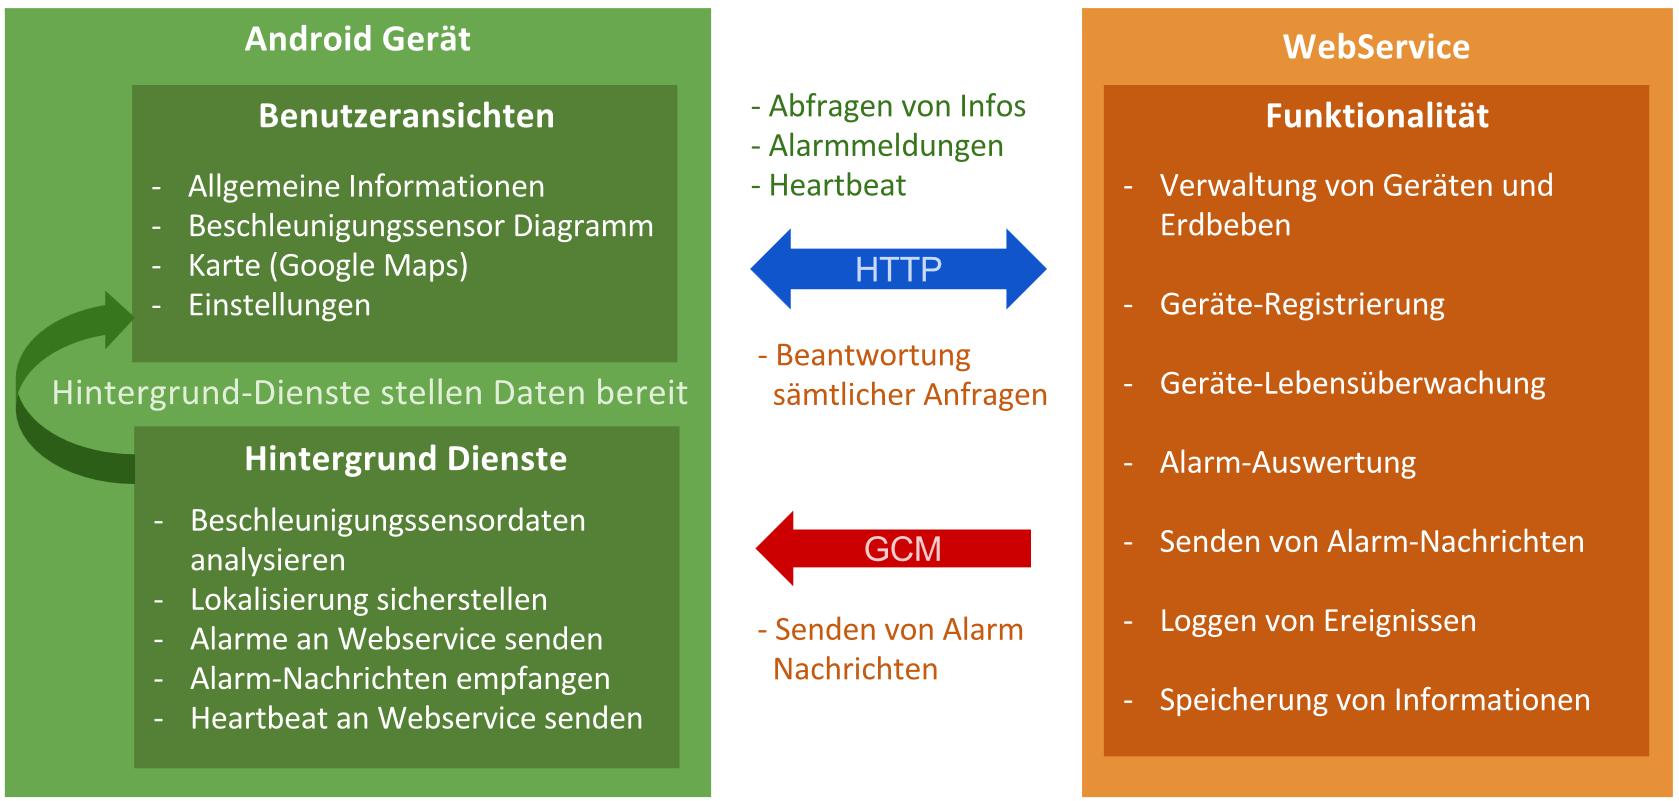
\includegraphics[width=\textwidth]{/Systemstruktur.png}
\caption{Struktur des Projektes}
\label{fig:SystemStrukutr}
\end{figure}
Das rechts dargestellte Android Gerät kann grundlegend in die Benutzeransichten und Hintergrund-Dienste unterteilt werden. 